% Intended LaTeX compiler: pdflatex
\documentclass[10pt,a4paper,UTF8]{article}
\usepackage{zclorg}
\author{zcl.space}
\date{}
\title{多天线高斯信道的容量}
\hypersetup{
 pdfauthor={zcl.space},
 pdftitle={多天线高斯信道的容量},
 pdfkeywords={communication algebra math},
 pdfsubject={本文总结差错控制编码第二章。},
 pdfcreator={Emacs 25.0.50.1 (Org mode 9.0.5)}, 
 pdflang={English}}
\begin{document}

\maketitle
\tableofcontents
\titlepic{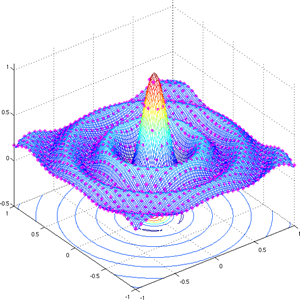
\includegraphics[scale=0.25]{../../img/sinc.PNG}}
\newpage


\section{系统模型}
\label{sec:org0539f85}
\begin{equation}
  \label{eq:20120322y}
  \mathbf{y} = H\mathbf{x} + \mathbf{n}
\end{equation}
where \(H\) is a \(r\times t\) matrix and \(\mathbf{n}\) is zero-mean complex Gaussian noise with independent, equal variance real and imaginary parts. We assume \(\mathcal{\mathbf{nn^{T}}}= I_r\) , that is the noises corrupting the different receivers are independent. The transmitter is constrained in its total power to \(P\) ,
\begin{equation}
  \label{eq:20120322varepsilon}
  \mathcal\{\mathbf{x}^{T} \mathbf{x}\} \le P
\end{equation}
因为 \(\mathbf{x}^{T}\mathbf{x} = tr(\mathbf{x}\mathbf{x}^{T})\) , and expectation and trace commute,
\begin{equation}
  \label{eq:20120322tr}
  tr(\mathcal{E}\{\mathbf{x}\mathbf{x}^{T}\}) \le P
\end{equation}
可以看出有功率限制和噪声分布限制。信道矩阵限制 \(H\) ,分三种情况:
\begin{enumerate}
\item \(H\)  is deterministic.
\item \(H\)  is a random matrix (for which we shall use the notation  \(\pmb{H}\)) , chosen according to a probability distribution, and each use of the channel corresponds to an independent realization of  \(\pmb{H}\) .
\item \(H\)  is a random matrix, but is fixed once it is chosen.

if \(Q\in \mathbb{C}^{n\times n}\) is non-negative devinite then so is \(\hat{Q}\in \mathbb{R}^{2n\times 2n}\) .
\end{enumerate}


The probability density(with respect to the standard Lebesgue measure on \(\mathbb{C}^{n}\) ) of a circularly symmetric complex Gaussian with mean \(\mu\) and covariance \(Q\) is given by 
\begin{eqnarray}
  \label{eq:20120323gamma}
  \gamma_{\mu,Q} &=& \det(\pi \hat{Q})^{-1/2} \exp(-(\hat{x} - \hat{\mu})^{T}\hat{Q}^{-1}(\hat{x} -\hat{\mu}) ) \nonumber \\
               &=& \det(\pi  {Q})^{-1/2} \exp(-( {x} -  {\mu})^{T} {Q}^{-1}( {x} - {\mu}) ) 
\end{eqnarray}

The differential entropy of a complex Gaussian \(\mathbf{x}\) with covariance \(Q\) is given by
\begin{eqnarray}
  \label{eq:20120323hgammaq}
  \mathcal{H}(\gamma_Q) &=& \mathcal{E}_{\gamma_Q}[-\log\gamma_Q(\mathbf{x})] \nonumber \\
                        &=& \log \det(\pi Q) + (\log e)\mathcal{E}[\mathbf{x}^{T}Q^{-1}\mathbf{x}] \nonumber \\
                        &=& \log \det(\pi Q) + (\log e)tr(\mathcal{E}[\mathbf{x}\mathbf{x}^{T}]Q^{-1}) \nonumber \\
                        &=& \log \det(\pi Q) + (\log e)tr(I)                 \nonumber \\
                        &=& \log \det(\pi eQ)
\end{eqnarray}
For us, the importance of the circulary symmetric complex Gaussians is due to the following lemma: circularly symmetric complex Gaussians are entropy maximizers. 

\begin{theorem}
Suppose the complex random vector \(\mathbf{x}\in \mathbb{C}^n\) is zero-mean and satisfied \(\mathcal{E}[\mathbf{xx}^{T}] = Q\) , i.e., \(\mathcal{E}[\mathbf{x}_i\mathbf{x}_j^*]=Q_{ij}, 1\le i,j \le n\)  then the ectropy of \(\mathbf{x}\) satisfies \(\mathcal{H}\le \log \det(\pi eQ)\) with equality if and only if \(\mathbf{x}\) is a circulary symmetric complex Gaussian with 
\begin{equation}
  \mathcal{E}[\mathbf{xx}^{T}] = Q
\end{equation}
\end{theorem}
\begin{proof}
Let \(p\) be any density function satisfying  \(\int_{\mathbb{C}^n} p(x)x_ix_j^* dx= Q_{ij}, 1\le j,j\le n\)  Let
\begin{equation}
    \label{eq:20120323gammaq}
    \gamma_Q(x) = \det(\pi Q)^{-1} \exp(-x^{T}Q^{-1}x).
\end{equation}
Observe that \(\int_{\mathbb{C}^n} \gamma_Q (x) x_ix_j^* dx = Q_{ij}\) , and that \(\log \gamma_Q(x)\) is  a linear combination of the terms \(x_ix_j^*\) . Thus \(\mathcal{E}_{\gamma Q}[\log\gamma_Q(\mathbf{x})]=\mathcal{E}_{p}[\log\gamma_Q(\mathbf{x})]\) . Then, 
\begin{eqnarray}
  \label{eq:20120323hpminushgammaq}
  \mathcal{H}_{p} - \mathcal{H}_{\gamma_Q} &=& -\int_{\mathbb{C}^n} p(x)\log{p(x)}dx + \int_{\mathbb{C}^n}  \gamma_Q(x)\log  \gamma_Q(x)dx \nonumber \\
     &=& -\int_{\mathbb{C}^n} p(x)\log{p(x)}dx + \int_{\mathbb{C}^n} p(x)\log  \gamma_Q(x)dx \nonumber \\
     &=& \int_{\mathbb{C}^n} p(x)\log \frac{ \gamma_Q(x)}{p(x)} dx \nonumber \\
     &\le&  0,
\end{eqnarray}
with equality only if \(p=\gamma_Q\) . Thus \(\mathcal{H}_{p} \le \mathcal{H}_{\gamma_Q}\)
\end{proof}

\begin{theorem}
if \(\mathbf{x}\in \mathbb{C}^n\) is a circularly symmetric complex Gaussian then so is \(\mathbf{y}=A\mathbf{x}\) , for any \(A\in \mathbb{C}^{m\times n}\) .
\end{theorem}

\begin{proof}
We may assume \(\mathbf{x}\)  is zero-mean. Let \(Q=\mathcal{E}[\mathbf{xx}^{T}]\) . Then \(y\) is zero-mean, \(\hat{\mathbf{y}} = \hat{A}\hat{\mathbf{x}}\) , and
\begin{equation}
   \mathcal{E}    [\hat{\mathbf{y}}\hat{\mathbf{y}}^{T}] = \hat{A} \mathcal{E}[\hat{\mathbf{x}}\hat{\mathbf{x}}^{T}]\hat{A}^{T} = \frac{1}{2} \hat{A}\hat{Q}\hat{A}^{T} =\frac{1}{2}\hat{K}.
\end{equation}
where \(K=\hat{A}\hat{Q}\hat{A}^{T}\).
\end{proof}

\begin{theorem}
if \(\mathbf{x}\) and \(\mathbf{y}\) are independent circularly symmetric complex Gaussians, then \(\mathbf{z} = \mathbf{x} + \mathbf{y}\) is a circulary symmetric complex Gaussian.
\end{theorem}
\begin{proof}
Let \(A=\mathcal{E}[\mathbf{xx}^{T}]\) and \(B=\mathcal{E}[\mathbf{yy}^{T}]\) . Then\(\mathcal{E}[\hat{\mathbf{z}}\hat{\mathbf{z}}^{T}]= \frac{1}{2}\hat{C}\) with \(C=A+B\)
\end{proof}

\section{具有固定传输函数的确定高斯信道}
\label{sec:org92b2ba7}

We will first derive an expression for the capacity \(C(H,P)\) of this channel, where \(H\in \mathbb{C}^{r\times t}\) . By the SVD theorem \(\mathbf{y} = H\mathbf{x}+ \mathbf{n}\) can be written as \(\mathbf{y}=UDV^{T}\mathbf{x}+\mathbf{n}\) , where \(D\in \mathbb{R}^{r\times t}\) .Let \(\tilde{\mathbf{y}} = U^{T}\mathbf{y}, \tilde{\mathbf{x}} = V^{T}\mathbf{x}, \tilde{\mathbf{n}} = U^{T}\mathbf{n}\) .Then, \(\tilde{\mathbf{y}} = D\tilde{\mathbf{x}} +\tilde{\mathbf{n}}\) . Since \(H\) is of rank at most \(\min\{r,t\}\) , at most  \(\min\{r,t\}\) of the singular values of it are non-zero. Denoting these by \(\lambda_i^{1/2},i = 1,2,\dots, \min\{r,t\}\) , we can write the matrix form of \(\tilde{\mathbf{y}} = D\tilde{\mathbf{x}} +\tilde{\mathbf{n}}\) component-wise, to get \(\tilde{y}_i = \lambda_{i}^{1/2}\tilde{x}_{i}+ \tilde{n}_{i}, \quad 1\le i \le  \min\{r,t\}\) , and the rest of the components of \(\tilde{y}\) (if any)are equal to the corresponding components of \(\tilde{n}\) . We thus see that \(\tilde{y}_{i}\) for \(i>  \min\{r,t\}\) is independent of the transmitted signal and that \(\tilde{x}_i\) for \(i> \min\{r,t\}\) don't play any role. To maximize the mutual information, we need to choose \(\{ \tilde{x}_i:1\le i \le  \min\{r,t\}\) to be independent, with each \(\tilde{x}_i\) having independent Gaussian, zero-mean real and imaginary parts. The variances need to be chosen via"water-filling" as
\begin{equation}
  \label{eq:20120323erexi}
  \mathcal{E}[\mathfrak{Re}(\tilde{x}_i)^2] =  \mathcal{E}[\mathfrak{Im}(\tilde{x}_i)^2]  = \frac{1}{2} (\mu -\lambda_i^{-1})^+
\end{equation}

where \(\mu\) is chosen to meet the power constraint. Here \(a^+\) denotes \(\max\{0,a\}\) . The power \(P\) and the maximal mutual information can thus be parameterized as
\begin{equation}
  \label{eq:20120323pmucmu}
  P(\mu) =\sum_{i} (\mu - \lambda_{i}^{-1})^+, \qquad C(\mu) =\sum_{i} (\ln (\mu\lambda_i))^+.
\end{equation}
\subsubsection{Alternative Derivation of the capacity} 
The mutual information \(\mathcal{I}(\mathbf{x};\mathbf{y})\) can be written as 
\begin{equation}
  \label{eq:20120323Ixy}
  \mathcal{I}(\mathbf{x};\mathbf{y}) = \mathcal{H}(\mathbf{y}) - \mathcal{H}(\mathbf{y}| \mathbf{x}) = \mathcal{H}(\mathbf{y}) - \mathcal{H}(\mathbf{n})
\end{equation}
and thus maximizing \(\mathcal{I}(\mathbf{x};\mathbf{y})\) is equivalent to maximizing \(\mathcal{H}(\mathbf{y})\) Note that if \(\mathbf{x}\) satisfies \(\mathcal{E}{\mathbf{x}\mathbf{x}^T}  \le P\) , so does \(x-\mathcal{E}[x]\) , so we can restrict our attention to zero-mean \(\mathbf{x}\) . Furthermore, if \(\mathbf{x}\) is zero-mean with covariance \(\mathcal{E}[\mathbf{x}\mathbf{x}^T] = Q\) , then \(\mathbf{y}\) is zero-mean with covariance \(\mathcal{E}[\mathbf{y}\mathbf{y}^T] = HQH^T + I_r\) , when the \(\mathbf{x}\) is circular symmetric complex Gaussian, the mutual information is given by:
\begin{equation}
  \label{eq:20120323Ixy2}
  \mathcal{I}(\mathbf{x};\mathbf{y}) = \log\det(I_r + HQH^T)= \log\det(I_r + QH^{T}H)
\end{equation}

where the second equality follows from the determinant identity \(\det(I+AB) = \det(I+BA)\) , and it only remains to choose \(Q\) to maximize this quantity subject to the constraints \(tr(Q)\le P\) and that \(Q\) is non-negative definite. Let \(\log\det(I+ HQH^{T})= \Psi(Q,H)\)
\subsection{Error Exponents}
\label{sec:org622ed69}

仅仅知道信道容量是不够的,通常还需要知道如何才能逼近这个容量,或者说,逼近这个容量的难度如何。于是,提出错误指数函数的概念给出差错概率一个上限。随机编码的上限是:
\begin{equation}
  \label{eq:20120323perror}
  \mathcal{P}(error) \le \exp(-nE_r(R))
\end{equation}
where the 随机编码的指数上限为:
\begin{equation}
  \label{eq:20120323err}
  E_r(R) = \max_{0\le \rho\le 1} E_0{\rho} -\rho R
\end{equation}
where, in turn, \(E_0{\rho}\) is given by supremum over all input distributions \(q_x\) satisfying the energy constraint of 
\begin{equation}
  \label{eq:20120323E0rhoqx}
  E_0(\rho, q_x) = -\log \int[\int q_x(x)p(y|x)^{1/(1+p)}dx]^{1+\rho} dy
\end{equation}
In our case \(p(y|x)=\det(\pi I_r)^{-1} \exp(-(y-x)^{T}(y-x))\) . If we choose \(q_x\) as the Gaussian distribution \(\gamma_Q\) we get (after some algebra).
\begin{equation}
  \label{eq:20120323E0rhoQ}
  E_0(\rho, Q) = \rho \log\det(I_r + (1+\rho)^{-1} HQH^{T}) = \rho\Psi((1+\rho)^{-1}Q,H)
\end{equation}

\subsection{Conclusion}
\label{sec:orgb8ac1f0}
The use of multiple antennas will greatly increase the achievable rates on fading channels if the channel parameters can be estimated at the reciver and if the path gains between different antenna pairs behave independently. The second of these requirements can be met with relative ease and is somewhat technical in nature. The first requirement is a rather tall order, and can be justified in certain communication scenarios and not in others. Since the original writing of this monograph in late 1994 and early 1995, there has been some work in which the assumption of the availability of channel state information is replaced with the assumption of a slowly varying channel.
\end{document}
